\documentclass[a4paper]{article}

\usepackage[portuguese]{babel}
\usepackage[utf8]{inputenc}
\usepackage{indentfirst}
\usepackage{graphicx}
\usepackage{verbatim}
\usepackage{wrapfig, blindtext}
\usepackage{listings}


\begin{document}

\setlength{\textwidth}{16cm}
\setlength{\textheight}{22cm}


\title{\Huge\textbf{LYNGK}\linebreak\linebreak\linebreak
\Large\textbf{Relatório Intercalar}\linebreak\linebreak
\linebreak\linebreak

\includegraphics[scale=0.1]{feup-logo.png}\linebreak\linebreak
\linebreak\linebreak
\Large{Mestrado Integrado em Engenharia Informática e Computação} \linebreak\linebreak
\Large{Programação em Lógica}\linebreak
		}

\author{
\textbf{Grupo LYNGK\_3:}\\
	Daniel Pereira Machado - up201506365 \\
	Sofia Catarina Bahamonde Alves - up201504570 \\
\linebreak\linebreak \\
 \\ Faculdade de Engenharia da Universidade do Porto \\ Rua Roberto Frias, s\/n, 4200-465 Porto, Portugal \linebreak\linebreak\linebreak
\linebreak\linebreak\vspace{1cm}}

\maketitle
\thispagestyle{empty}

\newpage

\section{Descrição detalhada do Jogo}
\subsection{História}

O LYNGK foi criado por Kris Burm, um designer de jogos, especialista em jogos de tabuleiro de estratégia abstrata, especialmente reconhecido pela coleção de jogos GIPF. Este projeto foi iniciado em 1998 com o lançamento do jogo que dá o nome à coleção, o próprio GIPF, e consistia em 6 jogos de tabuleiro. Mas, em 2017 foi lançado um novo jogo, o LYNGK, este jogo de tabuleiro é uma espécie de epílogo da coleção, pois resume todo o projeto, através da implementação dos elementos e das mecânicas que caraterizam cada um dos jogos da coleção.

\subsection{Conteúdo do jogo}

O jogo é constituído por 48 peças de 6 cores diferentes, cada uma relativa a um dos jogos da coleção. Existem 3 peças brancas (GIPF), 9 peças marfim (TZAAR), 9 peças azuis (ZÈRTZ), 9 peças vermelhas (DVONN), 9 peças verdes (PÜNCT) e 9 peças pretas (YINSH).

\subsection{Regras do jogo}

O objetivo do jogo é fazer conjuntos de 5 peças (stacks), cada um com 5 cores diferentes. O jogador com mais stacks  no final do jogo ganha.

\subsubsection{Preparação}

Colocam-se 8 peças de cada cor e 3 peças brancas de forma aleatório no tabuleiro, forma a que cada espaço que fique ocupado. As restantes peças ficam fora do tabuleiro, de forma a poderem ser escolhidas por um dos jogadores. Cada jogador apenas pode escolher 2 cores.

\subsubsection{Tipos de peças}

As 3 peças brancas são consideradas jokers, ou seja, podem representar qualquer uma das outras 5 cores ativas. Estas peças são passivas, isto é, não podem ser movidas por si mesmas, apenas como parte de uma stack.

No início do jogo todas as peças são neutras, não pertencem a nenhum jogador, assim podem ser movidas por qualquer um dos jogadores (com a exceção dos jokers). Ao longo do jogo cada jogador pode escolher 2 cores. Quando uma cor é escolhida as peças dessa cor deixam de ser neutras. A partir desse momento essas peças só podem ser movidas pelo jogador que escolheu a cor.

Os jogadores podem escolher cor em qualquer fase do jogo, mas devem fazê-lo no início da sua jogada, antes de moverem qualquer peça. Cada jogador só pode escolher uma cor de cada vez, não pode escolher 2 cores na mesma jogada. Quando ambos os jogadores tiverem escolhido 2 cores, a cor restante (a quinta cor) permanece neutra até ao final do jogo.


\subsubsection{Mover peças}

Os jogadores devem jogar alternadamente. Em cada jogada um jogador pode mover uma peça ou uma stack de peças. A cor da peça ou da stack deve fazer parte das cores escolhidas pelo jogador ou ser uma cor neutra.

Quando se trata de uma stack, esta deve ser sempre movida como um todo.  A peça que está no topo determina se a stack é neutra ou se pertence a um dos jogadores.

\begin{wrapfigure}{R}{0.3\textwidth}
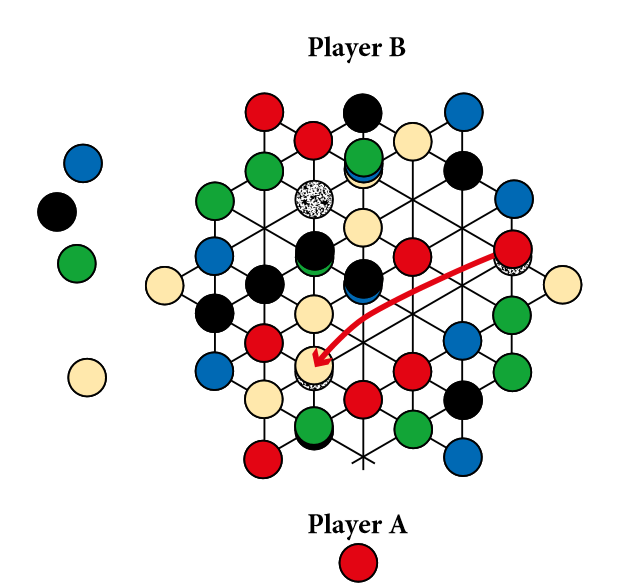
\includegraphics[width=0.3\textwidth]{board1.png}
\caption{\label{fig:Board1}O jogador A faz uma stack de 4 peças, as peças brancas podem assumir qualquer combinação de cores que não esteja na stack(verde, azul e preto).}
\end{wrapfigure}

Um movimento deve sempre acabar num espaço já ocupado, esteja lá uma peça ou uma stack. Os movimentos só podem ser feitos em linha reta, saltando apenas espaços vazios, não podem saltar por cima de peças. Ainda há outra opção de movimento, um movimento especial, que vai ser explicado na secção Regra-LYNGK.

Uma stack pode ter até 5 peças. O fundamento é que um conjunto apenas pode ser construído por peças de diferentes cores, isto é, não podem haver 2 peças da mesma cor na mesma stack. A exceção são as peças brancas, que ao poderem representar qualquer cor podem fazer parte dessa stack.

Uma peça neutra pode apenas ser movida para cima de outra peça. Por outras palavras, pode ser movida para cima de uma peça joker, de outra peça neutra, ou de uma peça de uma cor já escolhida pelo adversário. Uma peça nunca pode ser movida para cima de uma stack de peças.

Uma stack de peças com uma peça neutra no topo pode ser movida para cima de uma peça ou para cima de uma stack que tenha a mesma altura, ou uma altura inferior. Nunca pode ser movida para cima de uma stack com uma altura superior, ou seja, com  um maior número de peças. Por exemplo, uma stack de 2 peças pode ser movido para cima de outra stack de 2 peças, mas não para cima de uma de 3.

\begin{wrapfigure}{R}{0.3\textwidth}
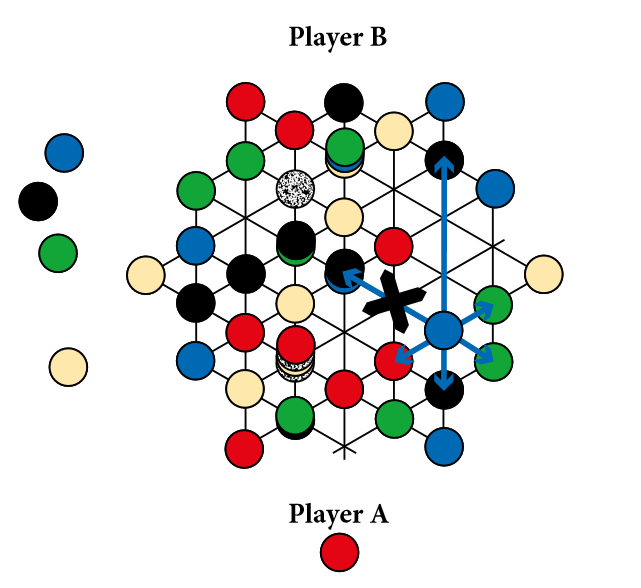
\includegraphics[width=0.3\textwidth]{board2.png}
\caption{\label{fig:Board2} A peça azul não pode fazer este moviemento porque a stack já possui uma peça azul e porque tem uma altura superior à peça.}
\end{wrapfigure}

Uma peça com cor escolhida ou uma stack que tenha uma peça de cor escolhida no topo pode ser movida para cima de qualquer peça ou stack (desde que a stack resultante não ultrapasse o máximo de 5 peças e as peças sejam todas de cores diferentes).

Quando um jogador completa uma stack de 5 peças com uma das cores escolhidas no topo do conjunto ele deve remover essa stack do tabuleiro e coloca-lo no seu lado. Uma stack removida vale um ponto no final do jogo.

Quando um jogador completa uma stack de 5 peças com uma cor neutra no topo, essa stack permanece no tabuleiro como obstáculo. Esta stack não conta como ponto para nenhum dos jogadores.

Não é permitido passar, a não ser que um jogador não consiga fazer mais nenhum movimento.

Caso um jogador não consiga fazer mais nenhum movimento o outro jogador continua a jogar até também não conseguir fazer mais nenhum movimento. Caso o jogador que passou volte a ter um movimento disponível pode continuar a jogar.


\subsubsection{Regra-LYNGK}

\begin{wrapfigure}{R}{0.3\textwidth}
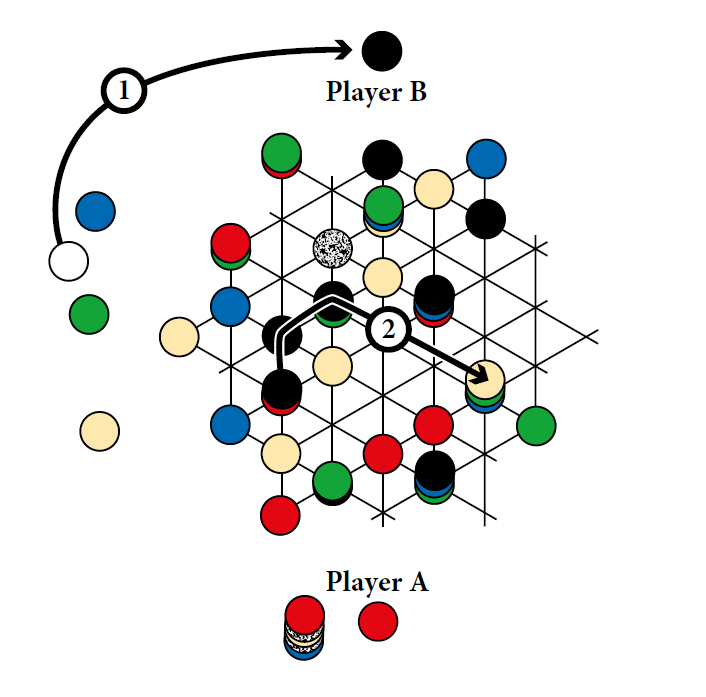
\includegraphics[width=0.3\textwidth]{lyngk-rule.png}
\caption{\label{fig:LYNGKrule} Exemplo de aplicação da regra-LYNGK}
\end{wrapfigure}

A regra LYNGK só pode ser aplicada quando se trata de uma cor escolhida. Esta regra diz que se duas peças da cor escolhida estiverem ligadas, ou seja, se for possível mover uma por cima de outra, pode-se fazer uma jogada especial. Deste modo é possível fazer uma jogada dupla, tripla, etc., usando a ligação entre esta peças.

Assim, quando se move uma peça para cima de outra da mesma cor, esta não deve permanecer aí, mas sim funcionar como um LYNGK-point, e fazer mais um movimento a partir daí. Se a peça for para cima de outra que também seja da cor escolhida deve ser repetido o mesmo princípio até chegar a uma peça que não seja da cor escolhida.

Não é permitido usar uma peça joker como LYNGK-point.
Em cada jogada só se pode usar este movimento uma vez.
NOTA: neste movimento só interessa a cor da peça ou do topo da stack, as restantes não são relevantes.

\subsubsection{Fim do jogo}

O jogo acaba quando é feita o último movimento possível. Vencedor é quem tiver o maior número de stacks com 5 cores diferentes.

No caso de empate, o vencedor é quem tiver o maior número de stacks de 4 peças no tabuleiro. Se continuar empatado verifica-se o mesmo para stacks de 3 peças e assim sucessivamente.

Se eventualmente, o número de peças isoladas for igual o jogo termina empatado.


\section{Representação do estado do jogo}

\small
\lstset{language=Prolog}
\lstinputlisting{initialBoard.pl}
\normalsize

\begin{wrapfigure}{R}{0.3\textwidth}
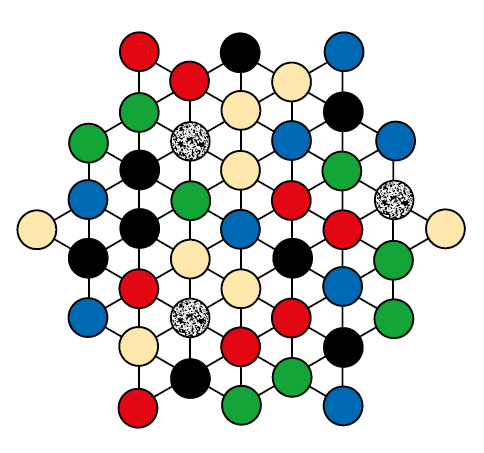
\includegraphics[width=0.3\textwidth]{initialBoard.png}
\caption{\label{fig:initialBoard} }
\end{wrapfigure}




\end{document}
